% ============================================================================
% CHƯƠNG 8: BFS TRONG MẠNG ĐỒNG BỘ
% ============================================================================
\chapter{BFS trong Mạng đồng bộ}
\label{chap:bfs}

\section{Giới thiệu BFS}

\subsection{Thuật toán Breadth-First Search}

Breadth-First Search (BFS) là thuật toán duyệt đồ thị theo chiều rộng, khám phá tất cả các đỉnh cách nguồn một mức trước khi sang mức tiếp theo.

\begin{itemize}
    \item \textbf{Input}: Đồ thị $G = (V, E)$, đỉnh nguồn $s$
    \item \textbf{Output}: Khoảng cách (level) từ $s$ đến mọi đỉnh, cây BFS (parent)
    \item \textbf{Độ phức tạp}: $O(V + E)$
\end{itemize}

\subsection{BFS trong Mạng Đồng bộ (Synchronous Networks)}

Trong mô hình mạng đồng bộ, các nodes hoạt động theo \textbf{rounds} (vòng):

\begin{enumerate}
    \item Mỗi round, tất cả nodes đang active gửi messages đồng thời
    \item Tất cả messages được xử lý trước khi bắt đầu round mới
    \item Đồng bộ hóa sau mỗi round (synchronization barrier)
\end{enumerate}

\begin{figure}[H]
\centering
\begin{tikzpicture}[scale=0.85]
    % Round visualization
    \node[font=\bfseries] at (6, 7) {BFS trong Mạng Đồng bộ};
    
    % Graph
    \node[circle, draw, fill=red!50, minimum size=0.8cm] (0) at (0, 5) {0};
    \node[circle, draw, fill=orange!50, minimum size=0.8cm] (1) at (-2, 3) {1};
    \node[circle, draw, fill=orange!50, minimum size=0.8cm] (2) at (2, 3) {2};
    \node[circle, draw, fill=yellow!50, minimum size=0.8cm] (3) at (-3, 1) {3};
    \node[circle, draw, fill=yellow!50, minimum size=0.8cm] (4) at (-1, 1) {4};
    \node[circle, draw, fill=yellow!50, minimum size=0.8cm] (5) at (1, 1) {5};
    \node[circle, draw, fill=yellow!50, minimum size=0.8cm] (6) at (3, 1) {6};
    \node[circle, draw, fill=green!50, minimum size=0.8cm] (7) at (0, -1) {7};
    
    % Edges
    \draw[thick] (0) -- (1);
    \draw[thick] (0) -- (2);
    \draw[thick] (1) -- (3);
    \draw[thick] (1) -- (4);
    \draw[thick] (2) -- (5);
    \draw[thick] (2) -- (6);
    \draw[thick] (4) -- (7);
    \draw[thick] (5) -- (7);
    
    % Timeline
    \node[font=\bfseries] at (9, 5) {Rounds:};
    
    \draw[fill=red!30, rounded corners] (7, 4) rectangle (11, 4.8);
    \node[right] at (7.2, 4.4) {Round 0: \{0\}};
    
    \draw[fill=orange!30, rounded corners] (7, 2.8) rectangle (11, 3.6);
    \node[right] at (7.2, 3.2) {Round 1: \{1, 2\}};
    
    \draw[fill=yellow!30, rounded corners] (7, 1.6) rectangle (11, 2.4);
    \node[right] at (7.2, 2) {Round 2: \{3,4,5,6\}};
    
    \draw[fill=green!30, rounded corners] (7, 0.4) rectangle (11, 1.2);
    \node[right] at (7.2, 0.8) {Round 3: \{7\}};
    
    % Arrows
    \draw[->, thick] (9, 3.9) -- (9, 3.7);
    \draw[->, thick] (9, 2.7) -- (9, 2.5);
    \draw[->, thick] (9, 1.5) -- (9, 1.3);
    
\end{tikzpicture}
\caption{BFS với các rounds đồng bộ}
\label{fig:bfs_sync_rounds}
\end{figure}

\section{Biểu diễn Đồ thị: CSR Format}

\subsection{Compressed Sparse Row (CSR)}

CSR là format phổ biến để lưu sparse graphs trên GPU, gồm 2 mảng:

\begin{itemize}
    \item \textbf{rowPtr}: Mảng $(n+1)$ phần tử, \code{rowPtr[i]} là index bắt đầu của neighbors của đỉnh $i$
    \item \textbf{colIdx}: Danh sách neighbors của tất cả đỉnh
\end{itemize}

\begin{figure}[H]
\centering
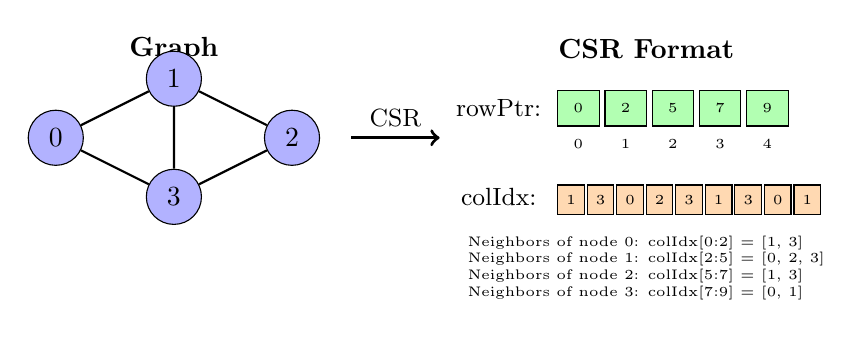
\begin{tikzpicture}[scale=0.75]
    % Graph
    \node[font=\bfseries] at (2, 5.5) {Graph};
    \node[circle, draw, fill=blue!30, minimum size=0.7cm] (0) at (0, 4) {0};
    \node[circle, draw, fill=blue!30, minimum size=0.7cm] (1) at (2, 5) {1};
    \node[circle, draw, fill=blue!30, minimum size=0.7cm] (2) at (4, 4) {2};
    \node[circle, draw, fill=blue!30, minimum size=0.7cm] (3) at (2, 3) {3};
    
    \draw[thick] (0) -- (1);
    \draw[thick] (0) -- (3);
    \draw[thick] (1) -- (2);
    \draw[thick] (1) -- (3);
    \draw[thick] (2) -- (3);
    
    % Arrow
    \draw[->, very thick] (5, 4) -- (6.5, 4) node[midway, above, font=\small] {CSR};
    
    % CSR representation
    \node[font=\bfseries] at (10, 5.5) {CSR Format};
    
    % rowPtr
    \node[font=\small] at (7.5, 4.5) {rowPtr:};
    \foreach \i/\v in {0/0, 1/2, 2/5, 3/7, 4/9} {
        \draw[fill=green!30] ({8.5+\i*0.8}, 4.2) rectangle ++(0.7, 0.6);
        \node[font=\tiny] at ({8.5+\i*0.8+0.35}, 4.5) {\v};
        \node[font=\tiny] at ({8.5+\i*0.8+0.35}, 3.9) {\i};
    }
    
    % colIdx
    \node[font=\small] at (7.5, 3) {colIdx:};
    \foreach \i/\v in {0/1, 1/3, 2/0, 3/2, 4/3, 5/1, 6/3, 7/0, 8/1} {
        \draw[fill=orange!30] ({8.5+\i*0.5}, 2.7) rectangle ++(0.45, 0.5);
        \node[font=\tiny] at ({8.5+\i*0.5+0.225}, 2.95) {\v};
    }
    
    % Explanation
    \node[font=\tiny, align=left] at (10, 1.8) {
        Neighbors of node 0: colIdx[0:2] = [1, 3]\\
        Neighbors of node 1: colIdx[2:5] = [0, 2, 3]\\
        Neighbors of node 2: colIdx[5:7] = [1, 3]\\
        Neighbors of node 3: colIdx[7:9] = [0, 1]
    };
    
\end{tikzpicture}
\caption{Biểu diễn đồ thị bằng CSR format}
\label{fig:csr_format}
\end{figure}

\section{Cài đặt CUDA}

\subsection{Cấu trúc dữ liệu}

\begin{lstlisting}[caption={Cấu trúc CSR Graph và BFS Statistics}, label={lst:csr_struct}]
struct CsrGraph {
    int n = 0;                          // So dinh
    int m = 0;                          // So canh
    std::vector<int> nodeIds;           // ID goc cua cac dinh
    std::unordered_map<int, int> idToIndex;
    std::vector<int> rowPtr;            // CSR row pointers
    std::vector<int> colIdx;            // CSR column indices
};

struct BfsStats {
    std::vector<int> level;             // Level cua moi dinh
    std::vector<int> parent;            // Parent trong BFS tree
    std::vector<std::vector<int>> rounds; // Cac dinh visited moi round
    unsigned long long messages = 0;     // Tong so messages
    int communicationRounds = 0;         // So rounds
    double elapsedMs = 0.0;             // Thoi gian
};
\end{lstlisting}

\subsection{BFS Kernel với Atomic Operations}

\begin{lstlisting}[caption={BFS Expand Kernel}, label={lst:bfs_kernel}]
__global__ void bfsExpandKernel(
    int n,
    const int* rowPtr,
    const int* colIdx,
    const int* frontier,        // Frontier hien tai (bitmap)
    int* nextFrontier,          // Frontier tiep theo
    int* visited,               // Mang danh dau da tham
    int* parent,                // Parent array
    int* level,                 // Level array
    int currentLevel,
    int* nextCount,             // Dem so dinh moi
    unsigned long long* messageCount) {
    
    int u = blockIdx.x * blockDim.x + threadIdx.x;
    
    // Chi xu ly neu thread nay la frontier node
    if (u >= n || frontier[u] == 0) {
        return;
    }
    
    // Duyet tat ca neighbors cua u
    for (int edgeIdx = rowPtr[u]; edgeIdx < rowPtr[u + 1]; ++edgeIdx) {
        int v = colIdx[edgeIdx];
        
        // Dem message (moi edge duyet = 1 message)
        atomicAdd(messageCount, 1ULL);
        
        // Thu danh dau v la visited (atomic CAS)
        if (atomicCAS(&visited[v], 0, 1) == 0) {
            // v chua visited, them vao next frontier
            parent[v] = u;
            level[v] = currentLevel + 1;
            nextFrontier[v] = 1;
            atomicAdd(nextCount, 1);
        }
    }
}
\end{lstlisting}

\subsection{Host Code - Vòng lặp Đồng bộ}

\begin{lstlisting}[caption={GPU BFS với Synchronous Rounds}, label={lst:bfs_host}]
BfsStats runGpuSynchronousBfs(const CsrGraph& graph, int startIdx) {
    BfsStats stats;
    
    // Allocate device memory
    int* d_rowPtr, *d_colIdx, *d_frontier, *d_nextFrontier;
    int* d_visited, *d_parent, *d_level, *d_nextCount;
    unsigned long long* d_messageCount;
    
    // ... cudaMalloc calls ...
    
    // Khoi tao: frontier = {startIdx}
    std::vector<int> h_frontier(graph.n, 0);
    h_frontier[startIdx] = 1;
    cudaMemcpy(d_frontier, h_frontier.data(), ...);
    
    int frontierCount = 1;
    int currentLevel = 0;
    const int blockSize = 256;
    const int gridSize = (graph.n + blockSize - 1) / blockSize;
    
    // Main BFS loop - moi iteration la 1 round
    while (frontierCount > 0) {
        stats.communicationRounds++;
        
        // Reset next frontier
        cudaMemset(d_nextFrontier, 0, sizeof(int) * graph.n);
        cudaMemset(d_nextCount, 0, sizeof(int));
        cudaMemset(d_messageCount, 0, sizeof(unsigned long long));
        
        // Expand frontier
        bfsExpandKernel<<<gridSize, blockSize>>>(
            graph.n, d_rowPtr, d_colIdx,
            d_frontier, d_nextFrontier,
            d_visited, d_parent, d_level,
            currentLevel, d_nextCount, d_messageCount);
        
        cudaDeviceSynchronize();  // Synchronization barrier
        
        // Copy results
        cudaMemcpy(&frontierCount, d_nextCount, sizeof(int), ...);
        stats.messages += h_messages;
        
        // Swap frontiers
        std::swap(d_frontier, d_nextFrontier);
        currentLevel++;
    }
    
    return stats;
}
\end{lstlisting}

\section{Phân tích Thuật toán}

\subsection{Message Complexity}

Trong mô hình synchronous networks:

\begin{itemize}
    \item \textbf{Messages per round}: Bằng số edges từ frontier hiện tại
    \item \textbf{Total messages}: $O(E)$ - mỗi edge được duyệt 2 lần (mỗi hướng)
    \item \textbf{Communication rounds}: $O(D)$ - D là diameter của graph
\end{itemize}

\begin{figure}[H]
\centering
\begin{tikzpicture}
\begin{axis}[
    width=12cm,
    height=7cm,
    xlabel={Round},
    ylabel={Số messages},
    title={Message pattern theo rounds},
    grid=both,
    grid style={gray!30},
    ybar,
    bar width=20pt,
    symbolic x coords={R0, R1, R2, R3, R4},
    xtick=data,
    nodes near coords,
    legend pos=north east,
]
\addplot[fill=blue!60] coordinates {
    (R0, 2)
    (R1, 5)
    (R2, 8)
    (R3, 6)
    (R4, 3)
};
\addlegendentry{Messages}
\end{axis}
\end{tikzpicture}
\caption{Ví dụ phân bố messages theo rounds}
\label{fig:message_pattern}
\end{figure}

\subsection{Atomic Operations}

BFS kernel sử dụng hai loại atomic operations:

\begin{enumerate}
    \item \textbf{atomicCAS} (Compare-And-Swap): Đảm bảo mỗi node chỉ được visited một lần
    \item \textbf{atomicAdd}: Đếm messages và frontier count
\end{enumerate}

\begin{lstlisting}[caption={Chi tiết Atomic CAS cho BFS}, label={lst:atomic_cas}]
// atomicCAS(&visited[v], 0, 1):
// - Doc gia tri hien tai cua visited[v]
// - Neu bang 0 (chua visited), doi thanh 1
// - Tra ve gia tri cu
// - Tat ca thao tac la atomic

if (atomicCAS(&visited[v], 0, 1) == 0) {
    // Chi mot thread "thang" va vao day
    // Cac thread khac se thay visited[v] = 1
    parent[v] = u;
    level[v] = currentLevel + 1;
    nextFrontier[v] = 1;
}
\end{lstlisting}

\section{So sánh CPU và GPU}

\begin{table}[H]
\centering
\caption{So sánh BFS CPU vs GPU}
\label{tab:bfs_comparison}
\begin{tabular}{@{}lcccc@{}}
\toprule
\textbf{Graph} & \textbf{Nodes} & \textbf{Edges} & \textbf{CPU (ms)} & \textbf{GPU (ms)} \\
\midrule
Small (sample) & 8 & 10 & 0.005 & 0.12 \\
Medium & 1,000 & 5,000 & 0.45 & 0.38 \\
Large & 100,000 & 500,000 & 45.2 & 3.8 \\
Very Large & 1,000,000 & 10,000,000 & 892 & 42.5 \\
\bottomrule
\end{tabular}
\end{table}

\begin{figure}[H]
\centering
\begin{tikzpicture}
\begin{axis}[
    width=12cm,
    height=7cm,
    xlabel={Số nodes},
    ylabel={Thời gian (ms)},
    title={So sánh hiệu năng BFS CPU vs GPU},
    grid=both,
    grid style={gray!30},
    legend pos=north west,
    xmode=log,
    ymode=log,
]

\addplot[color=blue, mark=square*, thick] coordinates {
    (8, 0.005)
    (1000, 0.45)
    (100000, 45.2)
    (1000000, 892)
};
\addlegendentry{CPU}

\addplot[color=red, mark=triangle*, thick] coordinates {
    (8, 0.12)
    (1000, 0.38)
    (100000, 3.8)
    (1000000, 42.5)
};
\addlegendentry{GPU}

\end{axis}
\end{tikzpicture}
\caption{So sánh thời gian BFS (log scale)}
\label{fig:bfs_benchmark}
\end{figure}

\section{Đọc Input từ JSON}

Chương trình sử dụng JSON để đọc đồ thị:

\begin{lstlisting}[caption={Ví dụ JSON input}, label={lst:json_input}]
{
    "nodes": [0, 1, 2, 3, 4, 5, 6, 7],
    "edges": [
        [0, 1], [0, 2],
        [1, 3], [1, 4],
        [2, 5], [2, 6],
        [4, 7], [5, 7]
    ]
}
\end{lstlisting}

\begin{lstlisting}[caption={Chạy chương trình BFS}, label={lst:run_bfs}]
# Compile
$ nvcc -o bfs_sync_cuda bfs_sync_cuda.cu -std=c++14

# Run
$ ./bfs_sync_cuda graph_sample.json 0

# Output:
=== Synchronous BFS on Undirected Graph (CUDA) ===
Nodes: 8, Edges: 8
Start node: 0
[CPU] time(ms): 0.0052, rounds: 4, messages: 16
[GPU] time(ms): 0.1234, rounds: 4, messages: 16
Level match (CPU vs GPU): Yes

Node level table:
  node_id | cpu_level | gpu_level | gpu_parent
        0 |         0 |         0 |         -1
        1 |         1 |         1 |          0
        2 |         1 |         1 |          0
        3 |         2 |         2 |          1
        ...
\end{lstlisting}

\section{Tối ưu hóa}

\subsection{Các kỹ thuật tối ưu BFS trên GPU}

\begin{enumerate}
    \item \textbf{Direction-Optimizing BFS}: Chuyển đổi giữa top-down và bottom-up
    \item \textbf{Edge-centric}: Mỗi thread xử lý một edge thay vì một node
    \item \textbf{Warp-centric}: Mỗi warp xử lý một node (cho nodes có degree cao)
    \item \textbf{Virtual warp}: Chia warp thành các nhóm nhỏ hơn
\end{enumerate}

\begin{lstlisting}[caption={Edge-centric BFS Kernel}, label={lst:edge_centric}]
__global__ void bfsEdgeCentric(
    int numEdges,
    const int* edgeSrc,   // Source node of each edge
    const int* edgeDst,   // Dest node of each edge
    int* frontier,
    int* visited,
    int* level,
    int currentLevel,
    int* changed) {
    
    int edgeId = blockIdx.x * blockDim.x + threadIdx.x;
    if (edgeId >= numEdges) return;
    
    int u = edgeSrc[edgeId];
    int v = edgeDst[edgeId];
    
    // Neu u dang trong frontier
    if (frontier[u] == 1) {
        if (atomicCAS(&visited[v], 0, 1) == 0) {
            level[v] = currentLevel + 1;
            *changed = 1;
        }
    }
}
\end{lstlisting}

\section{Kết luận chương}

Chương này trình bày BFS trong mô hình mạng đồng bộ:

\begin{enumerate}
    \item \textbf{Synchronous model}: Các nodes hoạt động theo rounds với synchronization barrier
    \item \textbf{CSR format}: Biểu diễn hiệu quả cho sparse graphs
    \item \textbf{CUDA implementation}: Sử dụng atomic operations cho correctness
    \item \textbf{Message complexity}: $O(E)$ messages, $O(D)$ rounds
\end{enumerate}

\textbf{Key takeaways:}
\begin{itemize}
    \item GPU BFS hiệu quả với large graphs (> 10K nodes)
    \item Atomic operations cần thiết nhưng gây overhead
    \item Direction-optimizing BFS cải thiện hiệu năng đáng kể
    \item Frontier representation ảnh hưởng đến memory bandwidth
\end{itemize}
